\chapter{Evaluation and Results}\label{evaluation-and-results}

This chapter reports what the pipeline actually does. It lays out the benchmark and the metrics, gives the headline comparison across all six configurations, then looks closer at where each one wins and loses, and finishes by testing whether the differences are real or just chance. What the numbers mean for the thesis is Chapter 6's business. Here the aim is narrower: state the results plainly.

\section{The benchmark}\label{the-benchmark}

Every number in this chapter rests on human judgement before it rests on any model. The benchmark is \textbf{1,748 messages}, each read and labelled by hand into one of the three classes, and every score reported below is a measurement of how closely a machine reproduces those human decisions. It is worth stating plainly what that means: the ground truth is not a downloaded label set but the outcome of reading 1,748 live chat messages one at a time, in the context each arrived in.

The messages come from live traffic on two platforms, 1{,}259 from YouTube and 489 from Twitch, spanning eleven domains from gaming and entertainment through to relationships and news.

They are also, by construction, the hard cases, and the reason bears restating. Sampling at random would have produced a benchmark with almost no positives in it: of the records taken at random for the control group, not one proved toxic once labelled. So the sampler weights its selection instead, as Section~\ref{datasets} describes, scoring each record on a toxic Tier-1 prediction, a disagreement between the tiers, and low Tier-1 confidence, then filling three quarters of the set from the top of that ranking and the last quarter at random from confidently-normal traffic. The result shows in the confidence distribution: Tier-1 confidence runs from 0.34 to 0.97 with a median of 0.64, and 1,536 of the 1,748 messages, 87.9 per cent, fall below the 0.80 escalation gate. The remaining 212 sit above the gate, and every one of them is a message Tier-1 called normal with high confidence, a median of 0.94. Two hundred and four of those are the random top-up; the other eight were pulled in because the two tiers had disagreed about them in spite of that confidence. So the benchmark is drawn from the second tier's own workload, with a control group of easy cases the judge should leave alone.

That 87.9 per cent describes how the benchmark was built, and it should not be mistaken for how often the pipeline escalates in ordinary running. The comparison worth making is against the collection run the benchmark was drawn from, since that holds the sampling effect apart from anything that changed between one run and another. That run captured 144,480 messages, and 8.3 per cent of them fell below the same 0.80 gate. Live chat is mostly confidently ordinary, so in normal operation the judge is called on roughly one message in twelve, against nearly nine in ten inside the benchmark. Earlier runs put the live figure between eight and fourteen per cent, so the exact rate moves with the streams being watched, but it stays an order of magnitude below the benchmark's in every case.

Of the 1,748, only \textbf{80 are toxic}, 59 offensive and 21 hateful. The other \textbf{1,668 are normal}. That is one toxic message in about twenty-two.

That ratio needs reading carefully, because two things follow from the same decision. Weighting the selection towards the hard cases is what put eighty positives in the set at all, and it is equally what stops the set standing in for ordinary traffic. Every score in this chapter therefore describes the pipeline on the difficult slice, not on an average hour of chat. What the weighting could not remove is the rarity of toxic content itself. Eighty against 1,668 is still a heavy imbalance, and having to cope with it is what rules out the obvious metric, as the next section explains.

Every configuration is scored against the same 1,748 labels, so the comparison is fair. Where a variant ran on only part of the set, from an earlier round of data collection, its score counts only the rows it covers, and that row count is reported next to it.

\section{Metrics}\label{metrics}

On a set this lopsided the tempting metric is accuracy, and it is easy to see why to avoid it. A model that ignored the text entirely and labelled everything ``normal'' would be right 1,668 times out of 1,748. Over 95 per cent accuracy, and not a single toxic message caught. Accuracy here rewards silence.

So the evaluation leads with the \textbf{toxic class} instead: precision, meaning of the messages flagged how many were truly toxic; recall, meaning of the truly toxic messages how many were caught; and F1, which combines the two. Three-class and binary accuracy still appear, but as background rather than headline.

The variants answer in different formats, so each verdict is first mapped to a common label, as Section~\ref{evaluation-methodology} describes. A memory verdict and a multi-agent verdict then get scored the same way against the same ground truth. Significance is checked with McNemar's test \citep{mcnemar1947}.

\renewcommand{\arraystretch}{1.5} 

\begin{longtable}{@{}
  >{\raggedright\arraybackslash}p{\dimexpr 0.1667\linewidth - 1.67\tabcolsep \relax}
  >{\raggedright\arraybackslash}p{\dimexpr 0.1667\linewidth - 1.67\tabcolsep \relax}
  >{\raggedright\arraybackslash}p{\dimexpr 0.1667\linewidth - 1.67\tabcolsep \relax}
  >{\raggedright\arraybackslash}p{\dimexpr 0.1667\linewidth - 1.67\tabcolsep \relax}
  >{\raggedright\arraybackslash}p{\dimexpr 0.1667\linewidth - 1.67\tabcolsep \relax}
  >{\raggedright\arraybackslash}p{\dimexpr 0.1667\linewidth - 1.67\tabcolsep \relax}@{}}
\caption{Per-variant results (n = 1,748).}\label{tab:headline}\tabularnewline
\toprule
\textbf{Variant} & \textbf{3-class acc} & \textbf{Binary acc} & \textbf{Toxic P} & \textbf{Toxic R} & \textbf{Toxic F1} \\
\midrule
\endfirsthead
\toprule
\textbf{Variant} & \textbf{3-class acc} & \textbf{Binary acc} & \textbf{Toxic P} & \textbf{Toxic R} & \textbf{Toxic F1} \\
\midrule
\endhead
\bottomrule
\endlastfoot

Tier-1 DistilBERT & 71.4\% & 72.0\% & 0.07 & 0.44 & 0.13 \\
\addlinespace[0.75em] % Separates the small baseline

Tier-2 baseline & 90.2\% & 91.0\% & 0.27 & 0.57 & 0.37 \\
\addlinespace[0.75em] % Separates the large baseline

Tier-2 + memory & 89.9\% & 90.6\% & 0.25 & 0.53 & 0.34 \\
Tier-2 + RAG & 90.6\% & 91.4\% & 0.27 & 0.51 & 0.35 \\
Tier-2 + LLM-Wiki & 88.3\% & 89.1\% & 0.23 & 0.57 & 0.33 \\
\addlinespace[0.75em] % Groups the isolated context strategies together

\textbf{Tier-2 multi-agent} & \textbf{92.6\%} & \textbf{93.2\%} & \textbf{0.33} & 0.47 & \textbf{0.39} \\

\end{longtable}
% Reset arraystretch to default for the rest of the document
\renewcommand{\arraystretch}{1.0}


One jump stands out above all the others: the step from Tier-1 to the Tier-2 baseline, where toxic F1 more than doubles from 0.13 to 0.37. Among the context modules the multi-agent setup leads clearly, on F1 at 0.39 and on both accuracy columns. The rest sit close to the baseline. The following sections take them one at a time.

\begin{figure}[H]
\centering
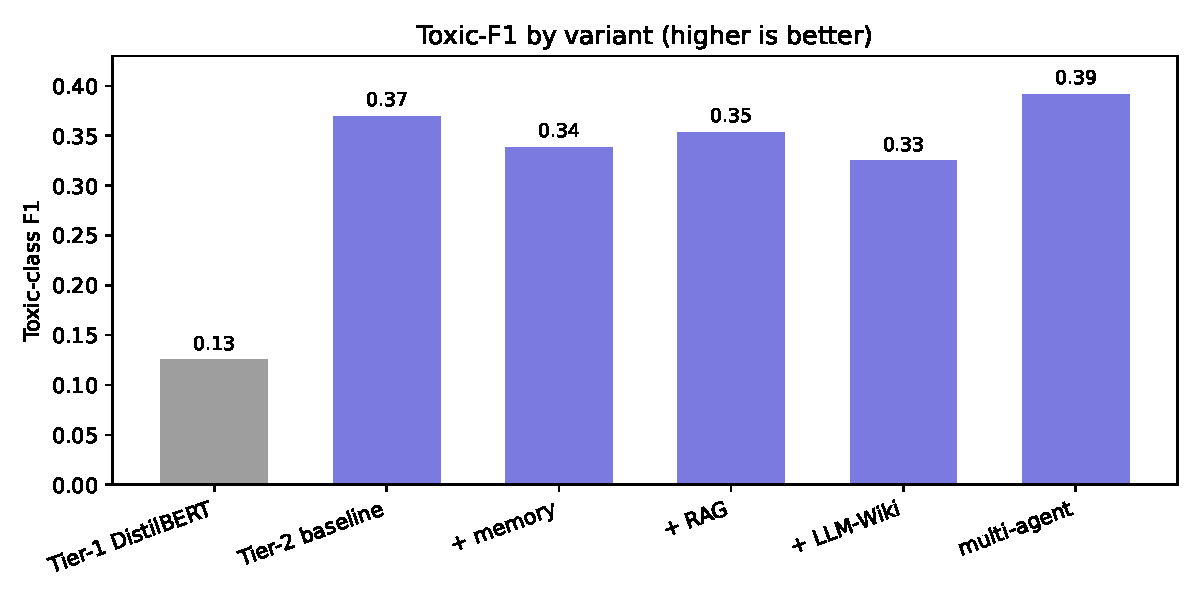
\includegraphics[width=0.9\linewidth,height=0.85\textheight,keepaspectratio]{figures/toxic_f1_by_variant.pdf}
\caption{Toxic-class F1 by variant. The two-tier baseline more than doubles Tier-1, and the multi-agent configuration leads the context variants.}\label{fig:toxicf1}
\end{figure}

\section{Reading the results}\label{reading-the-results}

\textbf{Tier-1 alone is a poor judge, and that is the point.} Its toxic F1 is 0.13 and its precision 0.07. Put plainly: when the static model shouts ``toxic,'' it is wrong roughly fourteen times out of fifteen. This is not a flaw. It is why the model sits first and not last, being fast, blind, good for surfacing suspects and useless as the final word. Those false alarms are exactly what the second tier is there to clean up.

\textbf{The two-tier design keeps its main promise.} Adding the LLM judge lifts toxic F1 from 0.13 to 0.37 and precision from 0.07 to 0.27. Behind the numbers, the judge is catching the static model's over-flagging: messages that look toxic to a word-counting model but read as ordinary in context, gaming trash talk, an angry but fair product review, get corrected. This answers RQ2, and it is the biggest effect in the study.

\textbf{Memory and RAG barely move the needle.} Memory nudges F1 down slightly, 0.37 to 0.34, and RAG down a touch to 0.35. Both stay next to the baseline. Knowing an author's recent history or seeing a handful of similar past cases simply did not change many verdicts here.

Section~\ref{why-memory-and-rag-stayed-neutral} goes into why this is happening, but the short answer is about the data and it can be quantified. The 1,748 messages come from 1,364 distinct authors. Of those, 1,134, or 83.1 per cent, appear exactly once, and the median author contributes a single message. A memory module asked to profile an author from one prior line has almost nothing to work with, and the same thinness limits the pool of past cases RAG can draw a close precedent from.

That is a limit of the data, not a mark against the context research. The most toxic content is deleted by moderators and automated filters before anyone can collect it, so the benchmark holds only eighty toxic messages, and the very cases these modules are built for are rare by nature. On a score driven by those eighty, a real gain on the normal majority hardly shows at all.

\textbf{The gap here is scarcity, not the modules themselves.} Splitting the set by collection order gives a partial check on that claim. Table~\ref{tab:scaling-toxic} scores the same variants first on the early subset, which held forty-four toxic messages, and then on the full eighty. Every configuration scores higher once the extra toxic examples arrive. The ordering stays inside the noise, and no context module overtakes the plain baseline at either size, so the headline conclusion is unchanged. But the direction is telling: as the toxic class grows, scores go up, not down. That is what a starved metric looks like, not a broken module, and it is the concrete reason the future-work chapter calls for growing the toxic class.

\begin{longtable}{@{}lll@{}}
\caption{Toxic-class F1 as the toxic set grows from 44 to 80 messages.}\label{tab:scaling-toxic}\tabularnewline
\toprule
Variant & F1 (44 toxic) & F1 (80 toxic) \\
\midrule
\endfirsthead
\toprule
Variant & F1 (44 toxic) & F1 (80 toxic) \\
\midrule
\endhead
\bottomrule
\endlastfoot
Tier-1 & 0.10 & 0.13 \\
Tier-2 baseline & 0.29 & 0.37 \\
Tier-2 + memory & 0.33 & 0.34 \\
Tier-2 + RAG & 0.27 & 0.35 \\
Tier-2 + LLM-Wiki & 0.28 & 0.33 \\
Tier-2 multi-agent & 0.35 & 0.39 \\
\end{longtable}

\textbf{The LLM-Wiki trades precision for recall, and loses the trade.} It matches the baseline on recall at 0.57, tied for the highest in the table, then drops to the lowest precision of any Tier-2 variant, 0.23, for an F1 of 0.33. The curated policy and glossary make the judge more suspicious. It catches as much toxicity as anything else and flags more innocent messages doing it, behaving rather like a moderator who has just read the rulebook cover to cover and now sees a violation everywhere.

\textbf{The multi-agent setup wins, and it wins by being careful rather than eager.} Its F1 of 0.39 is the best in the table. The shape of that win matters, though. It comes from the highest precision, 0.33, not the highest recall; its recall of 0.47 is in fact the lowest of the group. Splitting the decision across a risk scorer, a profiler, an escalator, and a supervisor produces a more cautious judge. It flags less. When it does flag, it is right more often.

\begin{figure}[H]
\centering
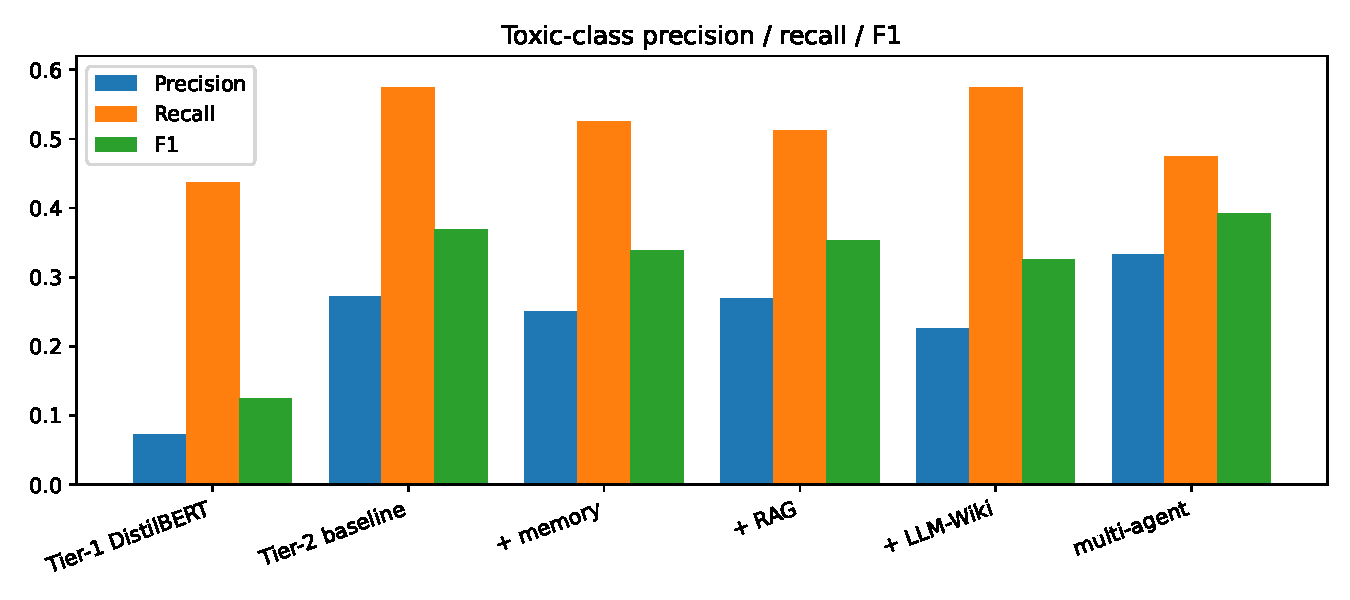
\includegraphics[width=0.9\linewidth,height=0.85\textheight,keepaspectratio]{figures/toxic_prf_by_variant.pdf}
\caption{Toxic-class precision, recall, and F1 side by side, showing the precision-recall trade-off each variant strikes.}\label{fig:toxicprf}
\end{figure}

\section{Inside the multi-agent chain}\label{inside-the-multi-agent-chain}

Each specialist writes its own signal to the record, so the winning variant can be opened up instead of treated as a black box. Doing that explains both what it achieved and what it did not. Table~\ref{tab:routing} gives the escalation router's decisions across the benchmark.

\begin{longtable}{@{}lll@{}}
\caption{Routing decisions made by the escalation agent (n = 1,748).}\label{tab:routing}\tabularnewline
\toprule
Action & Messages & Share \\
\midrule
\endfirsthead
\toprule
Action & Messages & Share \\
\midrule
\endhead
\bottomrule
\endlastfoot
Cleared automatically & 1,647 & 94.2\% \\
Flagged automatically & 57 & 3.3\% \\
Sent to human review & 44 & 2.5\% \\
\end{longtable}

Two things follow from that table.

First, the escalation path is live rather than ornamental. The router sent 44 messages to a person, flagged 57 on its own, and cleared the rest, which shows the three available actions are genuinely told apart instead of collapsing onto one default. The seam the design reserves for a human is therefore reached in practice, not merely declared. What it does not settle is the staffing question, and the gap between the two is wider than the figure suggests. One in forty is the rate inside the benchmark, and the benchmark is not ordinary traffic. Chaining the measured rates together gives a rough sense of the live equivalent: about eight per cent of messages reach the second tier at all, and about two and a half per cent of those are routed onward, which puts human review closer to one message in four hundred. Even that is an estimate rather than a measurement, and a generous one, since the benchmark's low-confidence portion is itself weighted towards difficult cases and will overstate how often the router reaches for a person. Whether any such load is workable then depends on arrival rate, on how long a reviewer needs per case, and on how many reviewers there are, none of which this study measures. The number shows the mechanism functions. Sizing it for a real moderation team is a separate exercise.

Second, and more interesting: the behaviour profiler returned low risk on \emph{every one} of the 1,748 records, covering 1,364 distinct authors. Not one came back medium or high. This is not a parse failure, since the chain falls back to ``medium'' when a response cannot be read. It is the profiler doing its job on data that gives it nothing. With 83.1 per cent of authors appearing exactly once, there is no pattern of prior behaviour to find, so the profiler correctly reports the absence of one, and the agent meant to contribute author history contributes a constant instead.

That sharpens how the multi-agent win should be read. The gain in precision cannot be coming from behavioural profiling, because that signal never varied at all. It comes from what is left: a risk score computed on content alone, a routing decision, and a supervisor forced to reconcile them. The same data sparsity that flattened memory and RAG also silenced one of the four agents, and the decomposition still won. Which suggests the benefit lies in splitting the judgement itself, rather than in any extra information the individual steps were supposed to supply.

\section{Confusion matrices}\label{confusion-matrices}

The confusion matrices in Figure~\ref{fig:confusion} show where the errors fall, not just how many there are. They tell the same story as the F1 column in a more concrete form. Tier-1's matrix is full of false positives in the top-right cell. The two-tier baseline shrinks that cell sharply. The Wiki variant lets it grow again as it over-flags. And the multi-agent matrix has the smallest false-positive cell of all, while still keeping a competitive count of true positives.

\begin{figure}[H]
\centering
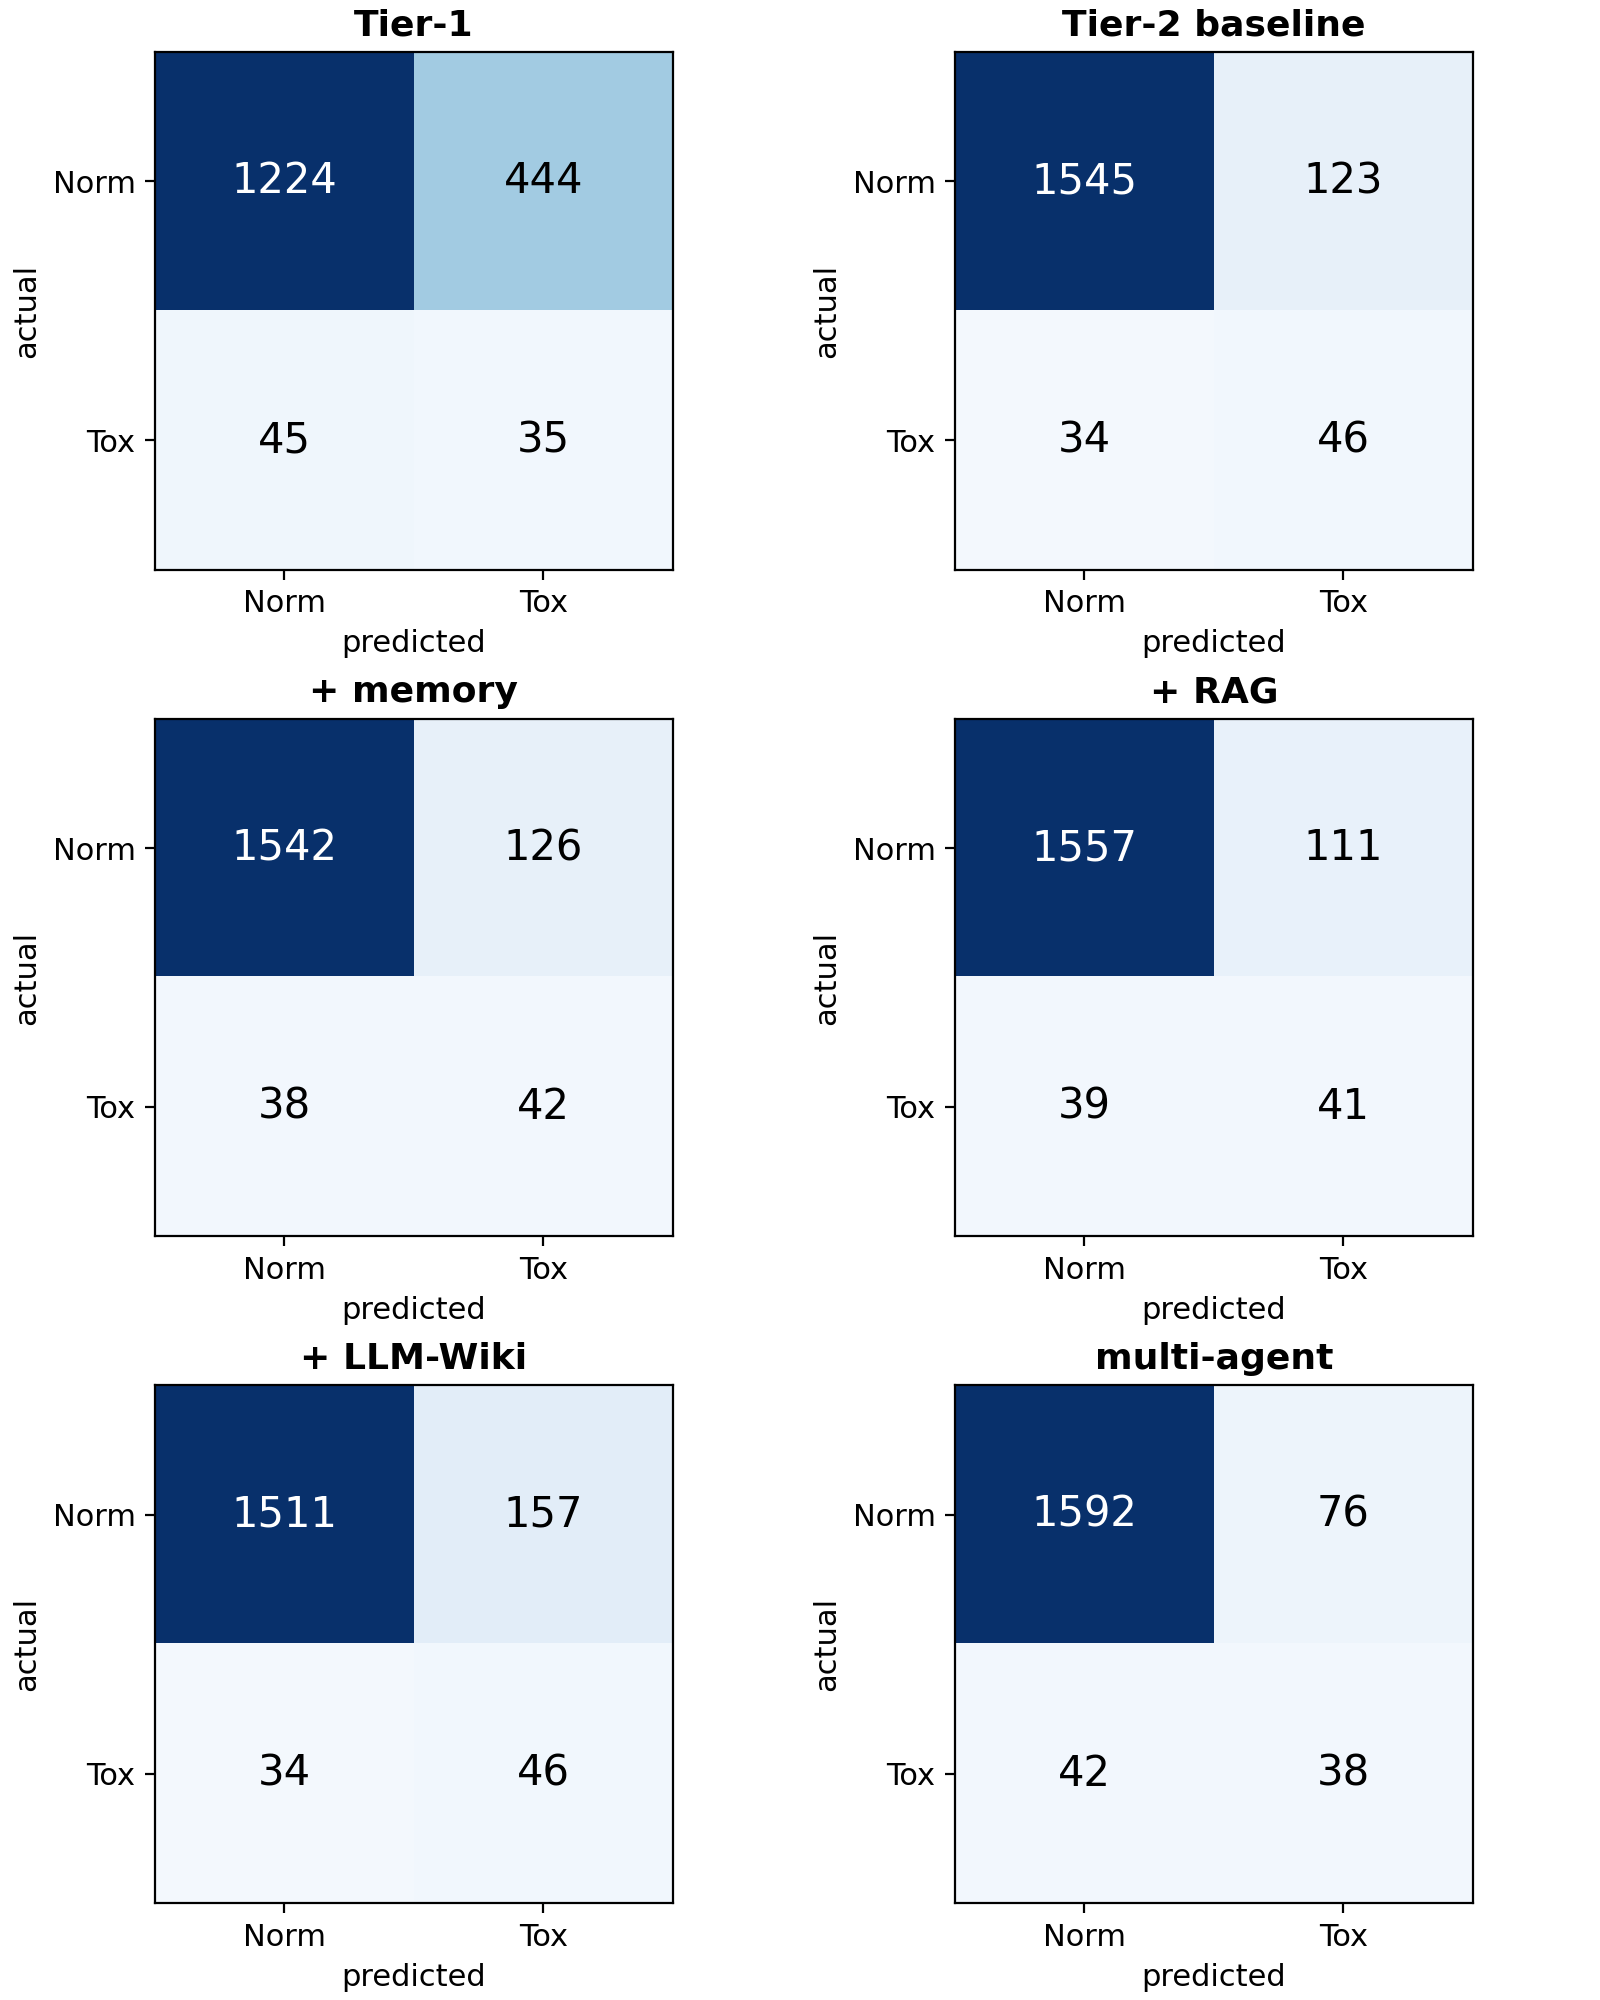
\includegraphics[width=0.9\linewidth,height=0.85\textheight,keepaspectratio]{figures/confusion_matrices_by_variant.png}
\caption{Binary confusion matrices per variant.}\label{fig:confusion}
\end{figure}

\section{Statistical significance}\label{statistical-significance}

With only 80 toxic messages, a handful of verdicts can swing an F1 score. So the real question is whether the gaps in Table~\ref{tab:headline} are solid. McNemar's test answers it by looking only at the messages where two systems disagree, then asking whether a variant fixes more of the baseline's mistakes than it creates. Table~\ref{tab:mcnemar} sets each variant against the Tier-2 baseline.

\begin{longtable}{@{}
  >{\raggedright\arraybackslash}p{\dimexpr 0.2000\linewidth - 1.60\tabcolsep \relax}
  >{\raggedright\arraybackslash}p{\dimexpr 0.2000\linewidth - 1.60\tabcolsep \relax}
  >{\raggedright\arraybackslash}p{\dimexpr 0.2000\linewidth - 1.60\tabcolsep \relax}
  >{\raggedright\arraybackslash}p{\dimexpr 0.2000\linewidth - 1.60\tabcolsep \relax}
  >{\raggedright\arraybackslash}p{\dimexpr 0.2000\linewidth - 1.60\tabcolsep \relax}@{}}
\caption{McNemar's test vs the Tier-2 baseline (toxic-vs-normal correctness).}\label{tab:mcnemar}\tabularnewline
\toprule
Variant & Baseline right, variant wrong & Variant right, baseline wrong & p-value & Verdict \\
\midrule
\endfirsthead
\toprule
Variant & Baseline right, variant wrong & Variant right, baseline wrong & p-value & Verdict \\
\midrule
\endhead
\bottomrule
\endlastfoot
+ memory & 63 & 56 & 0.582 & not significant \\
+ RAG & 52 & 59 & 0.569 & not significant \\
+ LLM-Wiki & 85 & 51 & \textbf{0.005} & significant, favours \textbf{baseline} \\
\textbf{multi-agent} & 40 & 79 & \textbf{\textless{} 0.001} & significant, favours \textbf{multi-agent} \\
\end{longtable}

Two results are significant, and they point in opposite directions.

The multi-agent system fixes 79 messages the baseline got wrong and breaks only 40. A genuine gain, not luck. The LLM-Wiki does the reverse: it changes many verdicts, 136 in all, more than any other variant, but the baseline is right on 85 of them against the Wiki's 51, so its over-flagging is a real effect rather than noise. Memory and RAG land in the middle, each disagreeing with the baseline about as often as it agrees, neither difference significant. Which is the statistical way of saying they neither helped nor hurt here.

\section{RAG versus the LLM-Wiki}\label{rag-versus-the-llm-wiki}

This is the head-to-head the two retrieval backends were built for.

On F1, vector RAG at 0.35 just edges out the curated-knowledge Wiki at 0.33, and they get there differently. RAG keeps the baseline's precision of 0.27 and trims recall. The Wiki keeps the baseline's recall and drops precision. Put simply: past cases nudged the judge toward caution, curated knowledge nudged it toward suspicion. Neither beat the plain baseline on this set, but the Wiki's effect was the larger of the two, and by Table~\ref{tab:mcnemar} the only significant one. Chapter 6 picks up what that says about the two ways of grounding a judge.

\begin{figure}[H]
\centering
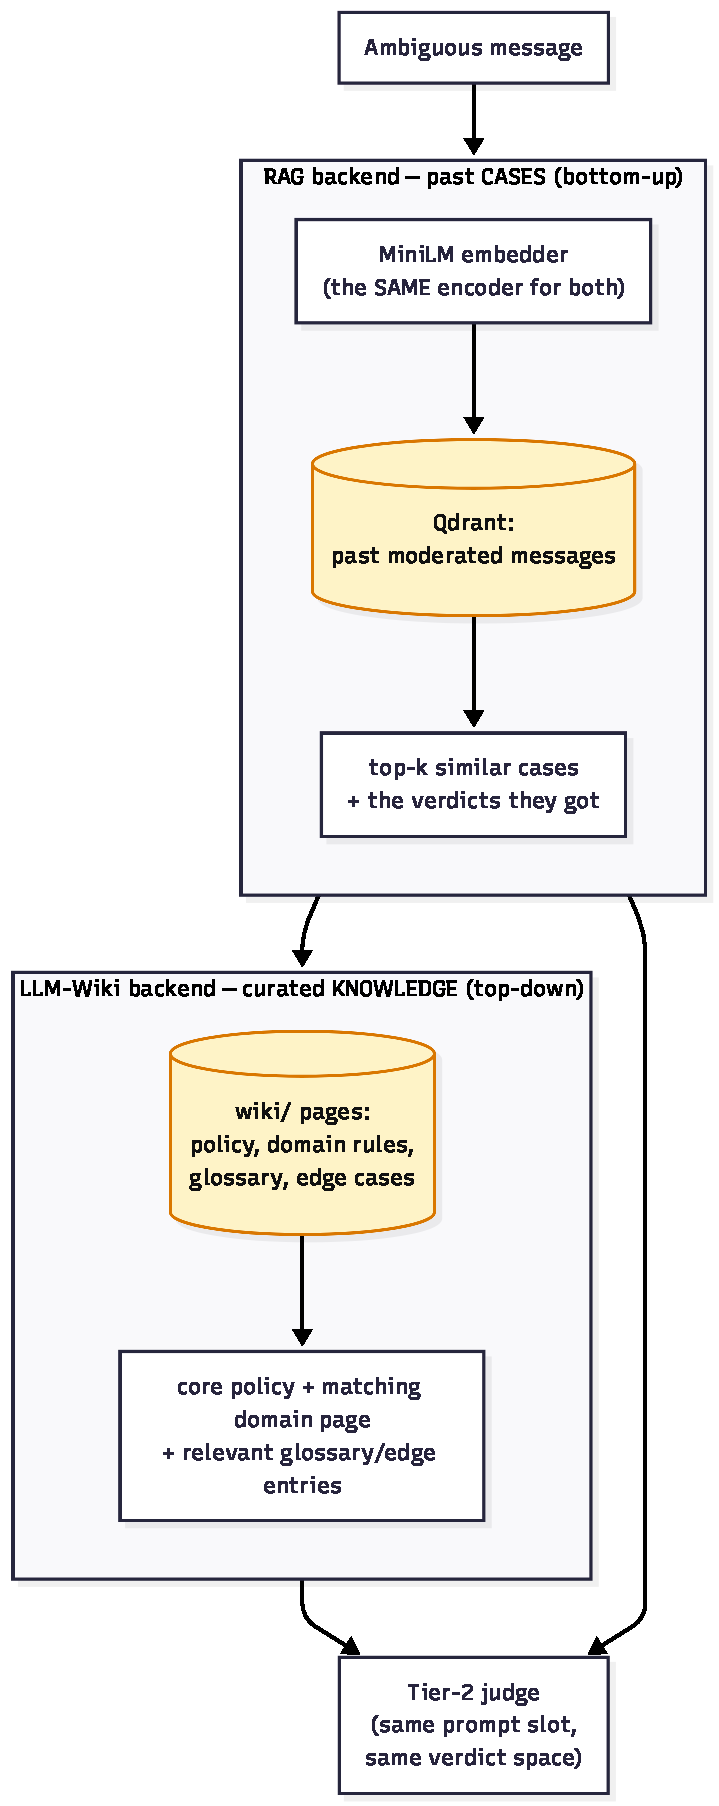
\includegraphics[width=0.9\linewidth,height=0.85\textheight,keepaspectratio]{figures/rag_vs_wiki.pdf}
\caption{RAG versus the LLM-Wiki: the two backends share the same embedder but draw on different corpora, RAG on past cases and the Wiki on curated knowledge, feeding the same judge in the same verdict space.}\label{fig:ragwiki}
\end{figure}

\section{Latency and computational cost}\label{latency-and-computational-cost}

Accuracy is only half the picture. What each verdict costs is the other half, and it is where the two tiers split most sharply. Table~\ref{tab:latency} has the timings.

\begin{longtable}{@{}lllll@{}}
\caption{Per-message latency for the two tiers.}\label{tab:latency}\tabularnewline
\toprule
Stage & Mean & Median & 95th pct & 99th pct \\
\midrule
\endfirsthead
\toprule
Stage & Mean & Median & 95th pct & 99th pct \\
\midrule
\endhead
\bottomrule
\endlastfoot
Tier-1 (DistilBERT) & 31 ms & 28 ms & 49 ms & 86 ms \\
Tier-2 (LLM judge) & 5.3 s & 4.6 s & 9.1 s & 12.8 s \\
\end{longtable}

Tier-1 labels a message in about 31 milliseconds. A single Tier-2 judgement takes about 5.3 seconds. That is a 174-fold gap, and it is the whole reason the second tier is used sparingly: running a five-second model on every message of a live stream is not an option, so it is saved for the low-confidence minority and run off the live path where it does not slow the stream.

The context modules add to that Tier-2 cost by different amounts, which matters when reading Table~\ref{tab:headline}. Memory adds a quick history lookup. RAG and the Wiki each add an embedding step and a search. The multi-agent setup makes four LLM calls instead of one, so it costs about four times the baseline judge, roughly twenty seconds a message. Table~\ref{tab:cost} puts cost next to benefit.

\begin{longtable}{@{}llll@{}}
\caption{Computational cost per message, by stage and variant.}\label{tab:cost}\tabularnewline
\toprule
Stage / variant & LLM calls & Typical latency & Toxic F1 \\
\midrule
\endfirsthead
\toprule
Stage / variant & LLM calls & Typical latency & Toxic F1 \\
\midrule
\endhead
\bottomrule
\endlastfoot
Tier-1 DistilBERT & 0 & 31 ms & 0.13 \\
Tier-2 baseline & 1 & 5.3 s & 0.37 \\
Tier-2 + memory & 1 (+ history fetch) & 5.3 s & 0.34 \\
Tier-2 + RAG & 1 (+ embed + search) & 5.5 s & 0.35 \\
Tier-2 + LLM-Wiki & 1 (+ embed + lookup) & 5.5 s & 0.33 \\
Tier-2 multi-agent & 4 & 21 s & \textbf{0.39} \\
\end{longtable}

Read together, that table changes how the multi-agent result looks. Its win on F1 is real and significant, and it comes at four times the cost of a single-shot judge. Any real deployment would have to decide whether the extra accuracy is worth the extra spend. The discussion of limits returns to this.

\section{Throughput, scalability, and resource use}\label{throughput-scalability}

Before the numbers, a word on how they were obtained, since a performance claim is only as good as its protocol. The latency figures in Table~\ref{tab:latency} are not estimates: the pipeline records the wall-clock time of every Tier-1 inference and every Tier-2 judgement as a field on the stored record, so the percentiles are computed over all 1,748 benchmark messages rather than sampled. Throughput was measured separately, by running the same fine-tuned classifier over messages drawn from the collected stream log in a loop, with a warm-up pass excluded and model loading timed apart from inference, and with Kafka and Elasticsearch out of the path so the figure reflects the model rather than the plumbing. Resource use was sampled once every two seconds during a sustained run, from the operating system and from the container runtime. All three are driven by scripts kept in the repository, so a reader can reproduce them on their own hardware and get a comparable set of numbers.

Latency is how long one message takes. Throughput is how many the pipeline handles per second, and it is the figure that decides whether the system can keep up with a live stream. Measured this way, Tier-1 handles about \textbf{thirty messages a second} on the single laptop used throughout, with full specifications in Appendix B. That is roughly 1,800 a minute, all on CPU. A busy live chat rarely runs past a few messages a second, so one machine has plenty of room to spare.

The raw rate matters, but so does whether it grows when compute is added. Table~\ref{tab:scaling} shows what happens as classifier processes are added, each pinned to one core. Throughput climbs, but by less each time, because one process already spreads across the laptop's four cores and they fill up fast. The real point is the direction, not the ceiling: adding compute adds throughput.

Two things should be said plainly about how far that extends. The deployment measured here runs Kafka with a single partition, so in the live pipeline exactly one Tier-1 consumer draws from the stream at a time; the numbers in Table~\ref{tab:scaling} come from running the classifier itself in parallel, which measures the compute tier rather than the full ingest path. Growing beyond one node therefore means raising the partition count first, after which consumers can be added on the same machine or on others with no change to producers, schema, or downstream code. That step is a configuration change, not a redesign, but it was not needed here and so was not measured. One node is capped by its cores; the architecture is not, and the distinction between what was measured and what follows from the design is drawn deliberately.

\begin{longtable}{@{}ll@{}}
\caption{Tier-1 throughput as CPU cores are added.}\label{tab:scaling}\tabularnewline
\toprule
Classifier processes & Throughput \\
\midrule
\endfirsthead
\toprule
Classifier processes & Throughput \\
\midrule
\endhead
\bottomrule
\endlastfoot
1 core & 17 msg/s \\
2 cores & 22 msg/s \\
4 cores & 25 msg/s \\
All cores, single process & 30 msg/s \\
\end{longtable}

Resource use under a steady load shows where the cost sits. Table~\ref{tab:resource} has the figures. Driving the classifier flat out pushes the CPU to its limit while the GPU stays almost idle, which confirms Tier-1 is CPU-bound, as expected for a small model run without GPU offload, and that the graphics card is not the bottleneck. Memory is the tighter limit on this machine. The containers themselves are cheap: Qdrant, Spark, Kafka, and Elasticsearch together use a fraction of a core and a few hundred megabytes while Tier-1 runs, because the heavy work is the model, not the plumbing.

\begin{longtable}{@{}ll@{}}
\caption{Resource use while Tier-1 runs under sustained load.}\label{tab:resource}\tabularnewline
\toprule
Component & Use under load \\
\midrule
\endfirsthead
\toprule
Component & Use under load \\
\midrule
\endhead
\bottomrule
\endlastfoot
Host CPU & 100\% peak, 88\% average \\
GPU & about 300 MB, under 10\% \\
Host memory & about 94\% \\
Containers (Kafka, Spark, Elasticsearch, Qdrant) & under 1\% CPU, a few hundred MB total \\
\end{longtable}

Put next to the latency figures, these answer RQ1 directly. The pipeline labels live messages from more than one platform at a median of 28 milliseconds and a steady thirty a second, on one modest laptop. For the target setting, that is real-time.

One distinction matters here more than anything else in the section, because only half of it has been tested. That throughput grows as cores are added is a measured result, and Table~\ref{tab:scaling} is the evidence for it. That the same would hold across separate machines is not. It follows from the architecture, since a partitioned log feeding stateless consumers is built to spread precisely that way, but a design supporting something and a thesis demonstrating it are different claims. Multi-node scaling is therefore recorded here as a capability the architecture provides and a validation still outstanding, not as a finding. Running that cluster benchmark is the obvious next step, and it belongs to future work rather than to this evaluation.

\section{Answering the research questions}\label{rq-summary}

The evidence in this chapter lines up with the three research questions, one row each. The design that motivated the study, from Chapters 3 and 4, fills the left of each row; this chapter fills the right. The path from question to answer can be followed straight across. Table~\ref{tab:rq} lays it out.

\renewcommand{\arraystretch}{1.5} 

\begin{longtable}{@{}
  >{\raggedright\arraybackslash}p{\dimexpr 0.07\linewidth - 1.6\tabcolsep \relax}
  >{\raggedright\arraybackslash}p{\dimexpr 0.25\linewidth - 1.6\tabcolsep \relax}
  >{\raggedright\arraybackslash}p{\dimexpr 0.22\linewidth - 1.6\tabcolsep \relax}
  >{\raggedright\arraybackslash}p{\dimexpr 0.26\linewidth - 1.6\tabcolsep \relax}
  >{\raggedright\arraybackslash}p{\dimexpr 0.20\linewidth - 1.6\tabcolsep \relax}@{}}
\caption{Each research question traced from design choice to experiment, evidence, and answer.}\label{tab:rq}\tabularnewline
\toprule
\textbf{RQ} & \textbf{Design choice} & \textbf{Experiment (metric)} & \textbf{Evidence} & \textbf{Answer} \\
\midrule
\endfirsthead
\toprule
\textbf{RQ} & \textbf{Design choice} & \textbf{Experiment (metric)} & \textbf{Evidence} & \textbf{Answer} \\
\midrule
\endhead
\bottomrule
\endlastfoot

\textbf{RQ1} & Partitioned Kafka log, decoupled tiers, per-platform adapters & Latency, throughput, scaling, resources (Sections~\ref{latency-and-computational-cost} and~\ref{throughput-scalability}) & 28 ms median, about 30 msg/s, rises with cores; two platforms, eleven domains & \textbf{Yes.} Real-time, multi-platform, easy to extend \\
\addlinespace[1em]

\textbf{RQ2} & Fast DistilBERT with a 0.80 confidence gate and a selective LLM auditor & Tier-1 vs Tier-2 baseline (Table~\ref{tab:headline}) & Toxic F1 from 0.13 to 0.37, precision from 0.07 to 0.27 & \textbf{Yes.} The study's largest effect \\
\addlinespace[1em]

\textbf{RQ3} & Temporal memory, RAG/Wiki, and multi-agent as switchable modules & Per-variant F1 and McNemar's test (Tables~\ref{tab:headline} and~\ref{tab:mcnemar}) & Multi-agent 0.39 (p \textless{} 0.001); memory and RAG not significant; Wiki significantly worse & \textbf{Partly.} Only the multi-agent decomposition helps \\

\end{longtable}
% Reset arraystretch to default for the rest of the document
\renewcommand{\arraystretch}{1.0}

RQ3 is the one qualified answer, and the qualification is the finding itself. Added context helps when it gives the decision structure, as the agent breakdown does. It does not help when it merely hands more information to a single judge.
